% Szglab4
% ===========================================================================
%
\chapter{Szkeleton tervezése}

\thispagestyle{fancy}

\section{A szkeleton modell valóságos use-case-ei}

\subsection{Use-case diagram}

\begin{figure}[h]
\begin{center}
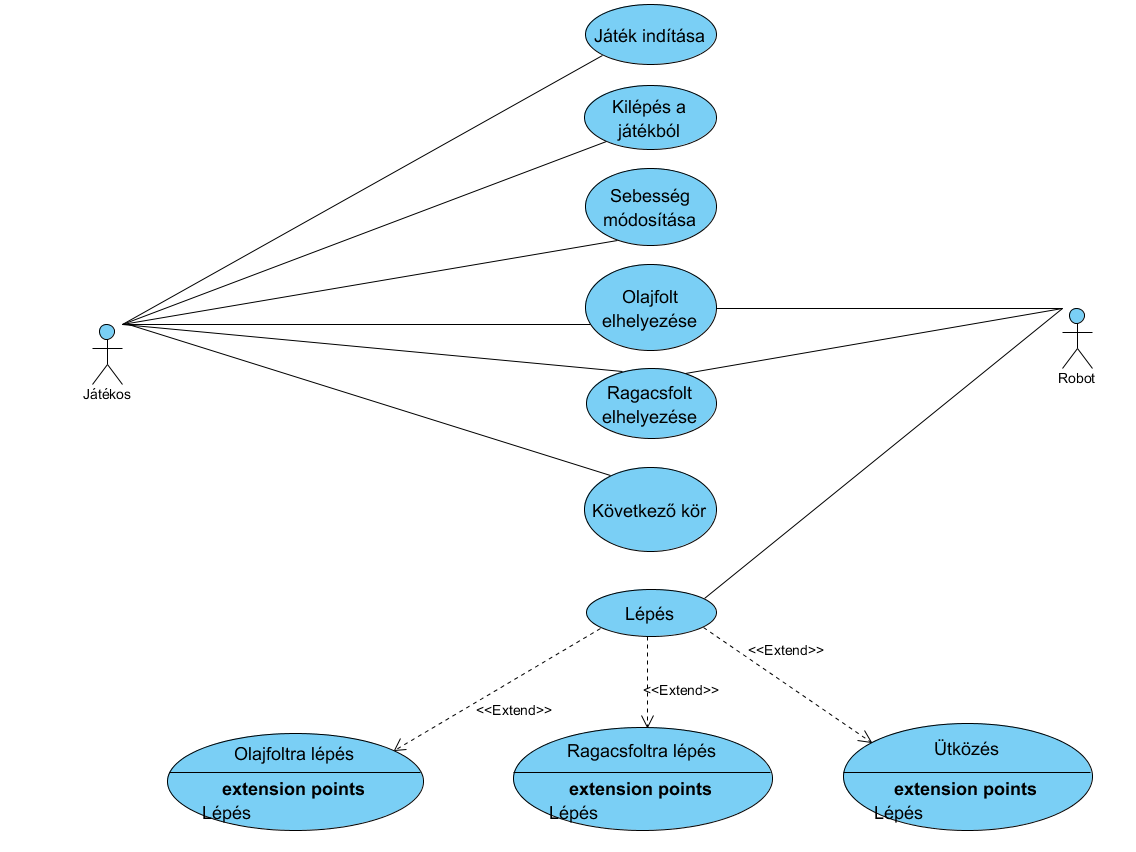
\includegraphics[width=17cm]{chapters/chapter05/use_case.png}
\caption{x}
\label{fig:SzkeletonUseCase}
\end{center}
\end{figure}

\subsection{Use-case leírások}



\usecase{Játék indítása}{Az egyik játékos elindítja a versenyt.}{Felhasználó}{A program menüjéből a felhasználó kiválasztja a Start game funkciót.}

\usecase{Kilépés a játékból}{A felhasználók ki tudnak lépni a játékból.}{Felhasználó}{Ha a játék közben egy játékos úgy dönt, hogy ki szeretne lépni, akkor ezt tudja jelezni és megsemmisül a hozzá tartozó robot.}

\usecase{Sebesség módosítása}{A robot sebesség vektora módosul.}{Játékos, Robot}{Egy játékos megváltoztatja saját robotjának a sebességét, tetszőleges irányú egységvektorral.}

\usecase{Olajfolt elhelyezése}{A robot egy olajfoltot hagy maga után.}{Játékos, Robot}{A játékos utasítására a robot elhelyez egy olajfoltot azon a cellán, amelyiken épp áll.}

\usecase{Ragacsfolt elhelyezése}{A robot egy ragacsfoltot hagy maga után.}{Játékos, Robot}{A játékos utasítására a robot elhelyez egy ragacsfoltot azon a cellán, amelyiken épp áll.}

\usecase{Következő kör}{Léptetés egy körrel.}{Játékos}{Ha minden játékos kiadta a kívánt utasításokat a robotoknak, akkor a kör befejeződik, s egy új kezdődik.}

\usecase{Kiesés a játékból}{Egy robot megsemmisülése.}{Robot}{Ha két robot ütközik, s nincs megfelelő cella számukra, akkor a két robot meghal és kiesik a játékból. Ha egy robot leugrik a kijelölt pályáról, akkor az szintén kiesik a játékból.}

\usecase{Játék megnyerése}{Egy robot megnyeri a játékot.}{Robot}{Ha egy robot marad már csak a pályán, akkor az a robot nyer. Ha elfogy a körök száma, akkor a legnagyobb távolságot megtett, életben maradt robot nyer.}

\usecase{Lépés}{A robot megteszi a lépését.}{Robot}{A robot tovább halad a pályán a megadott sebességvektorral.}

\usecase{Olajfoltra lépés}{A robot rálép egy olajfoltra.}{Robot}{Egy robot egy olajfoltos cellára kénytelen lépni, ezáltal a következő körben a sebessége nem módosítható.}

\usecase{Ragacsfoltra lépés}{A robot rálép egy ragacsfoltra.}{Robot}{Egy robot egy ragacsfoltos cellára kénytelen lépni, ezáltal a sebessége megfeleződik.}

\usecase{Ütközés}{A robotok ütköznek.}{Robot}{Két robot azonos cellára lép, így összeütköznek. Ha a robot egy olyan cellára lép, amelyen már áll egy robot, akkor az ott álló robot továbblép egy véletlenszerűen meghatározott szomszédos cellára. Ha nincs ilyen üres cella, akkor mindkét robot megsemmisül.}


\section{A szkeleton kezelői felületének terve, dialógusok}
A szkeleton egyes funkcióit egy menüből lehet majd elérni a parancssoron keresztül. A program indítása után megjelenik a főmenü a 8 menüponttal, amik közül a menüpont számának megadásával (és egy enter lenyomásával) választhat a felhasználó. A menü a következőképpen fog kinézni:\\

1. Játékindítás\\
\indent \hspace{1 cm}1.1 Cella hozzáadása\\
\indent \hspace{2 cm} 1.1.1 Cella koordinátái szóközzel elválasztva:\\
\indent \hspace{1 cm} 1.2 Robot hozzáadása\\
\indent \hspace{1 cm} 1.3 Főmenübe lépés\\
\indent 2. Robot sebességének módosítása\\
\indent \hspace{1 cm} 2.1 A sebesség koordinátái szóközzel elválasztva:\\
\indent 3. Olajfolt elhelyezése\\
\indent \hspace{1 cm} 3.1 Van olajfoltja a robotnak? $(I/N)$\\
\indent 4. Ragacsfolt elhelyezése\\
\indent \hspace{1 cm} 4.1 Van ragacsfoltja a robotnak? $(I/N$)\\
\indent 5. Következő kör\\
\indent \hspace{1 cm} 5.1 Ez volt az utolsó kör? $(I/N)$\\
\indent 6. Lépés\\
\indent \hspace{1 cm} 6.1 Üres sima cellára lép a robot\\
\indent \hspace{1 cm} 6.2 Ragacsos cellára lép a robot\\
\indent \hspace{1 cm} 6.3 Olajos cellára lép a robot\\
\indent \hspace{1 cm} 6.4 Pályán kívülre lép a robot\\
\indent 7. Ütközés\\
\indent \hspace{1 cm}	7.1 Van elég szabad hely a szomszéd cellákban? $(I/N)$\\	
\indent 8. Kilépés a játékból\\

Az almenüvel rendelkező menüpontok esetén a menüpont kiválasztása után megjelenik az almenü, aminek a kezelése a menüpontoktól függően változik. Abban az esetben, ha egy eldöntendő kérdést ír ki a program, akkor az $I$ billentyűvel adhat igenlő, az $N$ billentyűvel nemleges választ. Ha az almenü további menüpontokat tartalmaz, a főmenüből már ismert módon választhat közülük a felhasználó. (Csak a pont utáni részt szükséges beütnie.) Néhány esetben a program koordinátákat kér, ekkor egy szóközzel elválasztva kell megadni az $x$, majd az $y$ irányú koordinátát. A program itt egy-egy egész számot vár.\\
\par

A futások kimenete egy külső log fájlba fog kerülni, a felhasználó a konzolon keresztül csak arról fog visszajelzést kapni, hogy a végrehajtás részleteit a program kiírta ebbe a fájlba.\\
\par

A kimeneti fájlban az egyes futások elején megtalálható lesz a folyamat ami a konzolon a futtatás előtt lezajlott, valamint ezután az adott futás eredménye, azaz a meghívott függvények nevei. Ezek formátuma a következő lesz: $\left[ :ClassName\right].functionName(\left[ param \right]^*)$, ahol a $ClassName$ az adott osztály nevét, a $functionName$ a hívott függvény nevét, a $param$ kulcsszavak pedig egy-egy paramétert jelölnek. Felüldefiniált függvények esetén mindig a felüldefiniáló osztály neve íródik ki.



\section{Szekvencia diagramok a belső működésre}


\begin{figure}[!htbp]
	\begin{center}
		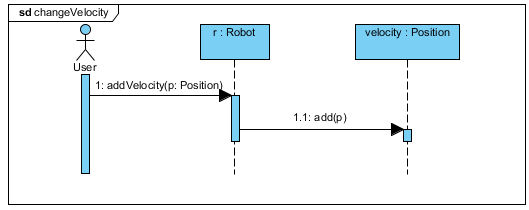
\includegraphics[width=13cm]{./chapters/chapter05/changevelocity.png}
		\caption{Sebesség módosítása}
	\end{center}
\end{figure}

\clearpage

\begin{figure}[!htbp]
	\begin{center}
		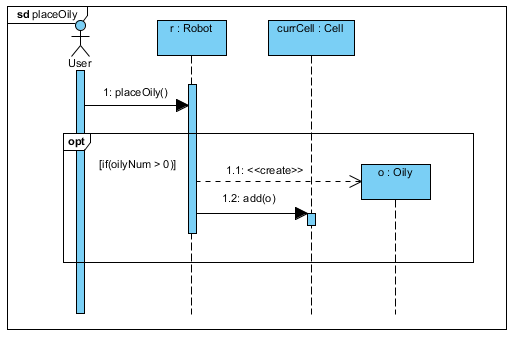
\includegraphics[width=13cm]{./chapters/chapter05/placeoilysequence.png}
		\caption{Olaj lerakása}
	\end{center}
\end{figure}

\begin{figure}[!htbp]
	\begin{center}
		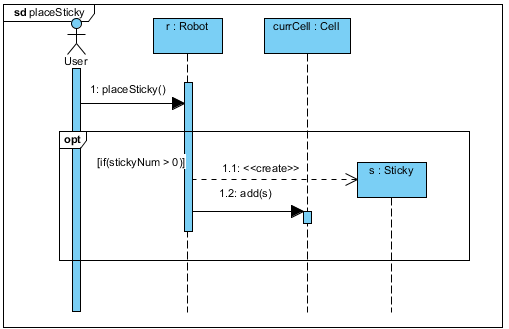
\includegraphics[width=13cm]{./chapters/chapter05/placestickysequence.png}
		\caption{Ragacs lerakása}
	\end{center}
\end{figure}

\clearpage

\begin{figure}[!htbp]
	\begin{center}
		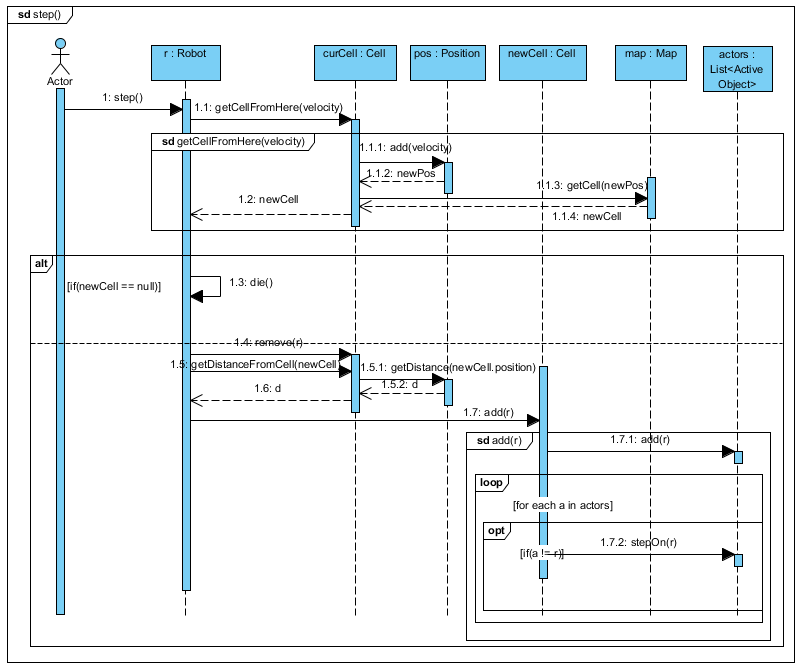
\includegraphics[width=18cm]{./chapters/chapter05/stepsequence.png}
		\caption{Lépés}
	\end{center}
\end{figure}

\clearpage

\begin{figure}[!htbp]
	\begin{center}
		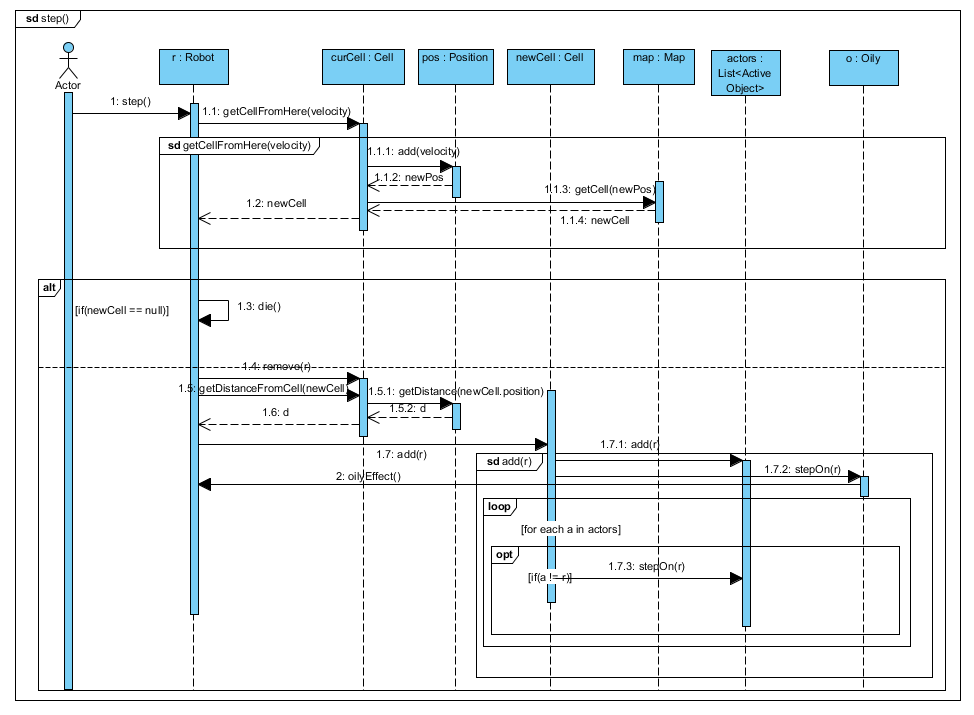
\includegraphics[width=18cm]{./chapters/chapter05/stepoilysequence.png}
		\caption{Lépés olajra}
	\end{center}
\end{figure}

\clearpage

\begin{figure}[!htbp]
	\begin{center}
		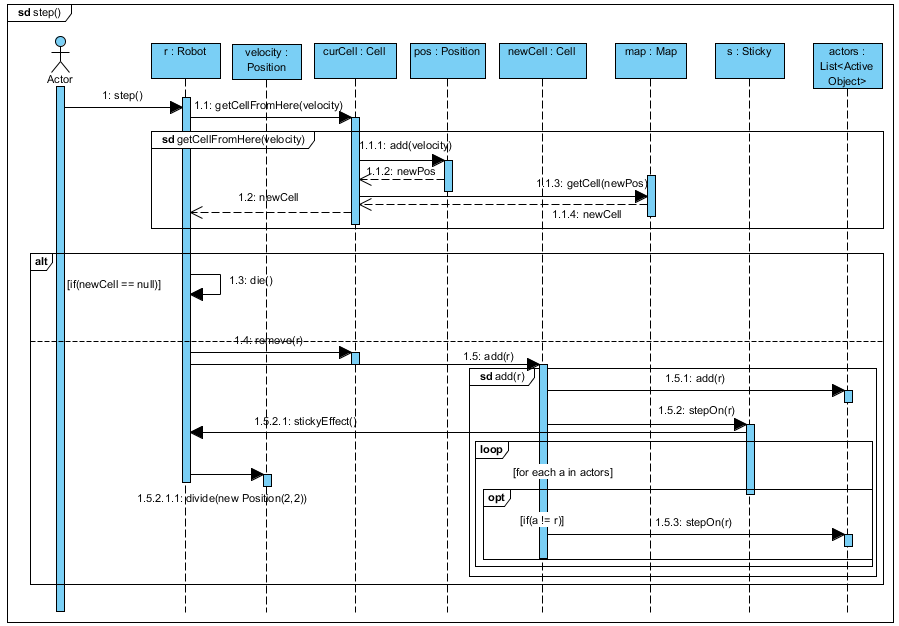
\includegraphics[width=18cm]{./chapters/chapter05/stepstickysequence.png}
		\caption{Lépés ragacsra}
	\end{center}
\end{figure}

\begin{figure}[!htbp]
	\begin{center}
		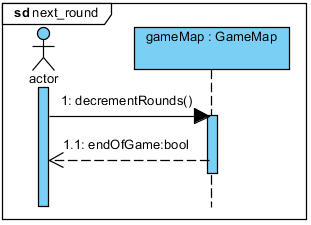
\includegraphics[width=6cm]{./chapters/chapter05/nextround.png}
		\caption{Következő kör}
	\end{center}
\end{figure}




\section{Kommunikációs diagramok}
\comment{A szkeletonban, az egyes szkeleton-use-case-ek futása során létrehozott objektumok és kapcsolataik bemutatására szolgáló diagramok. Ezek alapján valósítják meg a szkeleton fejlesztői az inicializáló kódrészleteket.}

\begin{figure}[!htbp]
	\begin{center}
		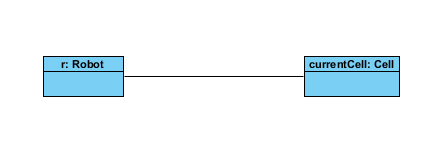
\includegraphics[width=13cm]{./chapters/chapter05/placetrapobject.png}
		\caption{Olajfolt / ragacsfolt lerakása}
	\end{center}
\end{figure}


\begin{figure}[!htbp]
	\begin{center}
		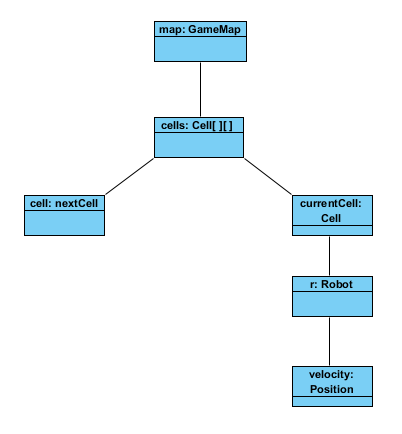
\includegraphics[width=13cm]{./chapters/chapter05/stepobject.png}
		\caption{Lépés, sebesség módosítása}
	\end{center}
\end{figure}
